%%%%%%%%%%%%%%%%%%%%%%%%%%%%%%%%%%%%%%%%%%%%%%%%%%%%%%%%%%%%%%%%%%%%%%%%%%

%%%%%                           Conclusion Géné                     %%%%%%
%%%%%%%%%%%%%%%%%%%%%%%%%%%%%%%%%%%%%%%%%%%%%%%%%%%%%%%%%%%%%%%%%%%%%%%%%%

\phantomsection 
\addcontentsline{toc}{chapter}{General conclusion} \mtcaddchapter
\addtocontents{toc}{\protect\addvspace{10pt}}

\vspace*{-1cm}
\begin{flushright}
\section*{\fontsize{20pt}{20pt}\selectfont\textnormal{General conclusion}}
\end{flushright}
\vspace{2cm}

\lhead[\fancyplain{}{General conclusion}]
      {\fancyplain{}{}}
\chead[\fancyplain{}{}]
      {\fancyplain{}{}}
\rhead[\fancyplain{}{}] 
      {\fancyplain{}{General conclusion}}
\lfoot[\fancyplain{}{}]
      {\fancyplain{}{}}
\cfoot[\fancyplain{}{\thepage}]
      {\fancyplain{}{\thepage}}
\rfoot[\fancyplain{}{}]
     {\fancyplain{}{\scriptsize}}

%%%%%%%%%%%%%%%%%%%%%%%%%%%%%%%%%%%%%%%%%%%%%%%%%%%%%%%%%%%%%%%%%%%%%%%%%%
%%%%%                      Start part here                          %%%%%%
%%%%%%%%%%%%%%%%%%%%%%%%%%%%%%%%%%%%%%%%%%%%%%%%%%%%%%%%%%%%%%%%%%%%%%%%%%

\section*{Outcomes}
The last few years have been very prolific for the field of markerless kinematics. Until recently, sport motion analysis had to be performed either with intrusive and complex marker-based techniques, or with rough and inaccurate markerless options. Nowadays, one can go without markers, and still obtain coherent 3D full-body joint kinematics. These methods are usually more robust than marker-based ones, and they are rapidly becoming more and more accurate. Our decision of crafting a robust triangulation procedure, and of constraining rough 3D coordinates to a biomechanically consistent skeletal model, makes it almost as accurate as marker-based solutions, at least for walking, running, and cycling. Such an approach has been proven to also work on-field, under constraints which make it difficult to set up a whole research-grade system. It is possible to use lightweight, wireless, consumer-grade cameras instead, although they are not straightforward to calibrate and synchronize. Equipment can also be detected along with the athlete, despite much like with marker-based techniques, inverse kinematics is not yet conclusive in case closed-loop constraints are enforced. Both in boxing and in BMX race, key performance indicators are retrieved satisfyingly. 

The workflow we proposed aimed at building a bridge between the computer vision and biomechanics communities, by using two of the most renown tools of their respective fields: OpenPose for 2D pose estimation, and OpenSim for 3D joint kinematics. This tool is open-source, versatile, and accessible for sports scientists who are the target audience, rather than computer vision specialists. As Pose2Sim was made to be useful and usable, it is also used: the University of Bath is currently creating a GUI around it, a (non-free) Blender add-on integrating it has been released \cite{Barreto2022}, and our GitHub repository is active. Pose2Sim has also been quoted by the University of Stanford, which later developed their own 3D markerless solution \cite{Uhlrich2022}. 

% \vskip 0.4cm

\section*{Limits and perspectives}
Some challenges remain, which would determine the adoption of markerless kinematic tools by the community of sports science. According to our most reported GitHub issues, the main stumbling block for users is calibration. Hence, there is definitively a need for an easier procedure, such as the one proposed by \cite{Argus}. It would even be worth testing an auto-calibration method, based on the knowledge of the size of a limb, tracked across multiple views. As we have demonstrated, an imperfect calibration does not degrade results much once 3D reconstruction constrained with a skeletal model has been applied. Moreover, the feedback given to athletes and coaches should be provided quickly enough for them to integrate it, so that they can adjust their motion patterns before their next trial sequence. Quasi-real-time can be achieved with research-grade cameras, as videos are directly downloaded after each sequence on the master computer, which can run Pose2Sim in the background. For wireless consumer-grade cameras, it is more complicated, although downloading media can sometimes be done remotely, without risking impairing camera calibration. Additionally, by essence, team sports are practiced as a group, and thus performing multi-person inverse kinematics can be important. Although we did not implement it yet, we described methods to achieve such a task. Finally, sports scientists are usually more at ease with graphical user interfaces than with command line, and coaches prefer an intuitive visual feedback rather than charts of joint angle waveforms. A visualization tool for Maya has been developed, but it is not yet ready for release. Moreover, as all the tools used and proposed here are open-source, it would make more sense to propose it as a free standalone software application, or as a Blender add-on (see Figure~\ref{fig_blendermocap} for planned features, and Figure~\ref{fig_mayamocap} for those already developed on the Maya-MoCap toolbox). Furthermore, this work gave rise to a projected collaboration with the University of Bath, which is currently developing a GUI for Pose2Sim, and with whom we plan to build a new sports dataset for more accurate markerless kinematics. 

% \vskip 0.4cm

\section*{Future prospects}
Current datasets for 2D pose estimation are not accurately labelled, they suffer from a dearth of keypoints, and they are not trained to recognize sports poses nor any equipment. Building a whole new dataset could solve these issues. The dataset should be large and diverse enough, represent a wide variety of body types and of sports movements \cite{Seethapathi2019}, and include images with motion blur such as found in sports videos. The images in this dataset should not include any markers, since they could be interpreted as visual cues, which are not available in real sports situations. And yet, they should be labelled accurately. One way to do it is to build a synthetic dataset. 

For example, a mass of .c3d motion files could be gathered from various sports, and be used to fit an SMPL+H mesh \cite{Pavlakos2019}, for example with AMASS \cite{Mahmood2019}. These data could be augmented with already existing datasets for daily life activities, such as Agora \cite{Patel2021}. Multiple persons should be present in the scene, using sports equipment. Then, random clothing, background, light could be added (see \cite{Wood2021,Bolanos2021} for a detailed workflow), as well as variations in SMPL shape parameters. Numerous virtual cameras could then be placed in the scene, in order to gather a large amount of diverse perspective points.

Labelling human beings could theoretically be done on one single SMPL mesh. Hence, the SMPL topology is constant, and one could assume that the positions of these virtual markers on the mesh would be consistently propagated to other frames, other poses, and other body shapes. This labelling technique could be termed "virtual palpation". As many virtual markers as needed could be used, for a precise evaluation of any movement and pose. However, only an expert should perform this task, and make sure that markers are correctly positioned: crowd-sourcing this task, like it is done for more basic image classification and segmentation with ImageNet \cite{Deng2009}, has been proved to lead to systematic offset errors \cite{Needham2021b}. Finally, 3D virtual markers could be automatically projected on the 2D camera planes. This would result in an extensive sports dataset, created with minimal labelling work, on a potentially infinite amount of views. 

Nevertheless, before training the network, one should make sure that the generated data is as diverse as the real world, by using one of the metrics proposed by \cite{Borji2019, Borji2022}. Additionally, keypoint positions need to be precise enough: SMPL shape vertices can sometimes be more than 5 cm apart, which could cause imprecision errors similar to skin artifacts. 


\begin{figure}[hbtp]
      \centering
      \Rotatebox{-90}{
      \def\svgwidth{1\columnwidth}
      \fontsize{10pt}{10pt}\selectfont
      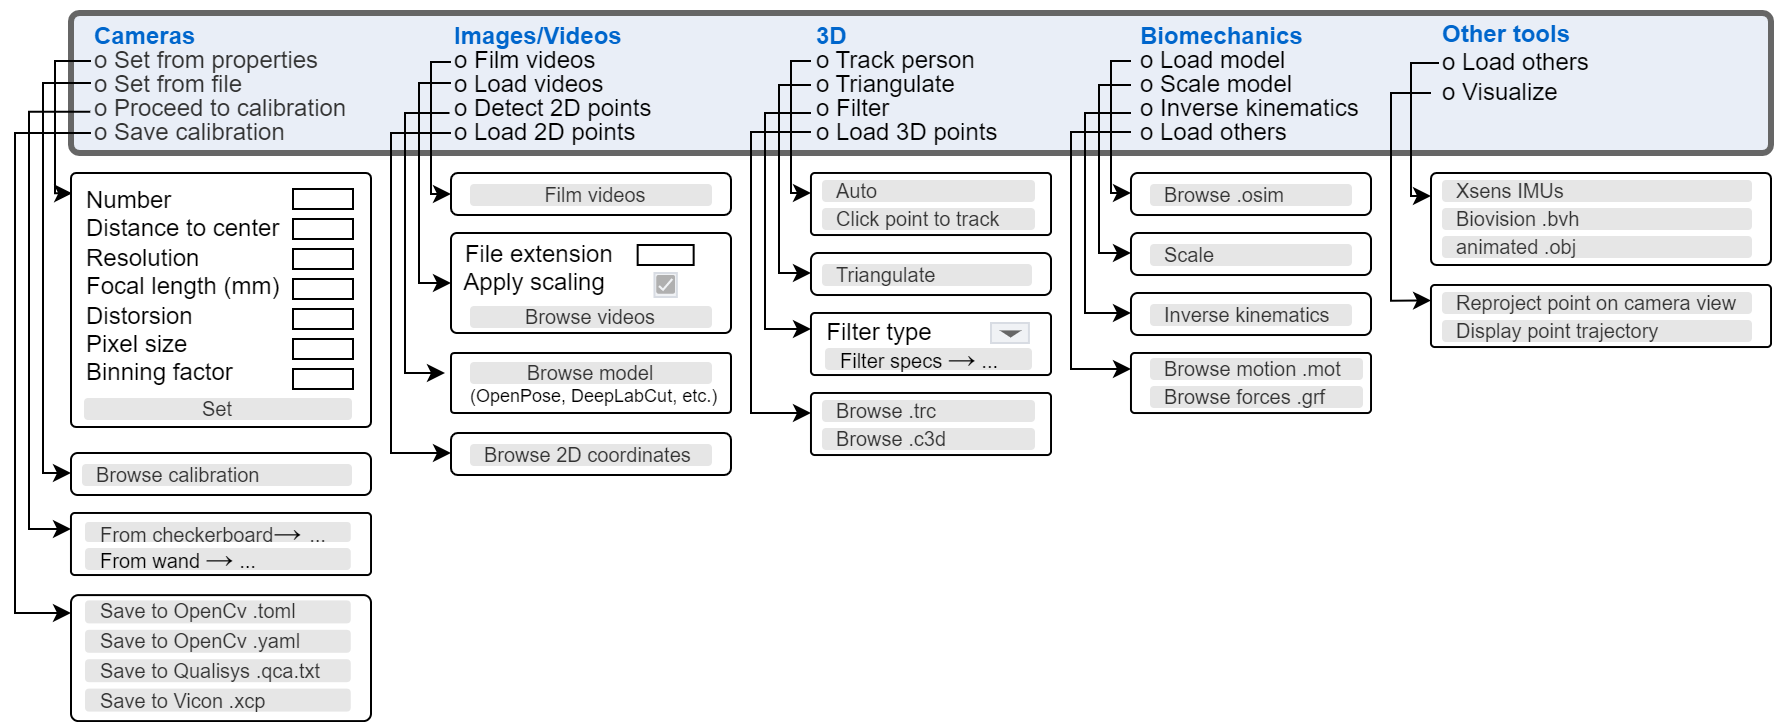
\includegraphics[height=0.6\linewidth]{"../Chap3/Figures/Fig_MayaMocap3.png"}}
      \caption{Planned features of the future Blender add-on. See Figure~\ref{fig_mayamocap} for reference to the already developed Maya-Mocap add-on.}
      \label{fig_blendermocap}
\end{figure}




% marche course vélo bmx boxe chill nage danse (lancer, parkour?)